\documentclass{standalone}
\usepackage{tikz}
\usetikzlibrary{patterns}
\usepackage{pgfplots}
\begin{document}%
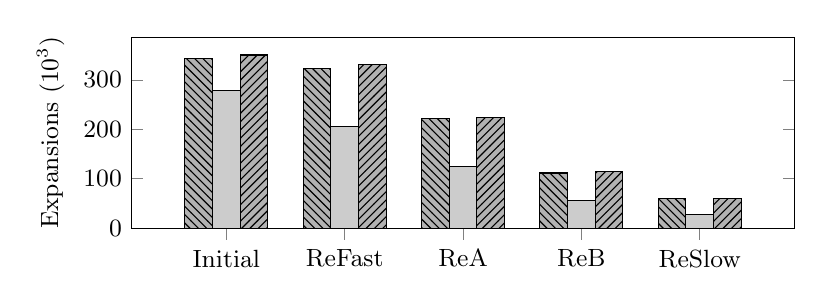
\begin{tikzpicture}[font=\small]

% this stats are currently manually computed
% from results of experiment: Makefile.incbi-road-ne


\begin{axis}[
   ybar=0pt,
   %bar width=0.20cm,
   enlarge x limits=0.2,
   width=10cm, height=4cm,
   ymin=0,
   ylabel={Expansions ($10^3$)},
   xlabel near ticks,
   ylabel near ticks,
   xtick=data,
   symbolic x coords={Initial,ReFast,ReA,ReB,ReSlow},
   xtick pos=left,
   ]

% lpastar
\addplot+[draw=black,fill=black!30,postaction={pattern=north west lines}]
coordinates
{
   (Initial,342.307755)
   (ReFast,323.0747175) % pblock = 0.0010
   (ReA,222.00896138888889) % pblock = 0.0005
   (ReB,111.56027138888888) % pblock = 0.0002
   (ReSlow,59.14850027777778) % pblock = 0.0001
};

% incbi
\addplot+[draw=black,fill=black!20]
coordinates
{
   (Initial,277.9990225)
   (ReFast,206.19699694444446) % pblock = 0.0010
   (ReA,124.36986944444444) % pblock = 0.0005
   (ReB,55.84239638888889) % pblock = 0.0002
   (ReSlow,28.027845833333333) % pblock = 0.0001
};

% rlpastar
\addplot+[draw=black,fill=black!30,postaction={pattern=north east lines}]
coordinates
{
   (Initial,350.20625)
   (ReFast,331.56562555555557) % pblock = 0.0010
   (ReA,224.65325444444444) % pblock = 0.0005
   (ReB,114.67884694444445) % pblock = 0.0002
   (ReSlow,60.82335083333333) % pblock = 0.0001
};

\end{axis}

\end{tikzpicture}%
\end{document}
